% set 0.5 inch indentation
\setlength{\parindent}{0in}
% set paragraph space = 0 space
\setlength{\parskip}{1.5mm}
% set line space 1.5
\setlength{\baselineskip}{1.6em}

\chapter{INTRODUCTION}
\section{Background}

In computer vision, self-distillation \shortcite{furlanello2018born, zhang2019your, xie2020self} is a technique for improving deep learning models without increasing model size.
This paradigm involves training a student model whose parameter size is equal to the teacher model with new parameter initialization.
One method from this paradigm can work without any label called Self-\textbf{di}stillation with \textbf{no} labels (DINO) \shortcite{caron2021emerging}.
The method has been shown to improve the performance of both ResNet \shortcite{he2016deep} and Vision Transformers (ViT) \shortcite{dosovitskiy2021an}.
According to \shortciteA{allen-zhu2023towards}, when using the self-distillation technique, the student model is forced to learn soft-label features, which were extracted from the dataset. Additionally, by training the model with difference parameter initialization, the student model acquires knowledge from multiple views of images. The result shows around 2\% improvement by the self-distillation method over multiple ResNet models \shortcite{Zagoruyko2016WideResnet}.

% However, most self-distillation methods have conventionally focused on visual information without using the textual information, which can be concise and informative.
% By utilizing text and image information, the model can learn to extract semantic information from the images based on text description.
In another branch of research, a multimodal approach demonstrates that the model's performance can be improved when combining both image and text data into the model.
Contrastive Language-Image Pre-training (CLIP) \shortcite{radford2021learning} and \textbf{A} \textbf{L}arge-scale \textbf{I}ma\textbf{G}e and \textbf{N}oisy-text embedding (ALIGN) \shortcite{jia2021scaling} both achieved performance on par with fully supervised image classification across multiple benchmarks.
These models are obtained by training the models with image-text pairs using the contrastive vision language pre-training method.
The current state-of-the-art is \textbf{Co}ntrastive \textbf{Ca}ptioner (CoCa) \shortcite{yu2022coca}.
This approach used image-text pairs with contrastive language-image loss and image captioning loss.
Thus, it is a clear benefit of the training model in utilizing image and text information.
% Thus, this work investigated the effectiveness of using both texts and images with the self-distillation method.

\begin{figure}[h]
    \caption{Overall methodology}
    \label{fig:overall_method}
    Self-distillation training with image text joined representation.
    \begin{center}
        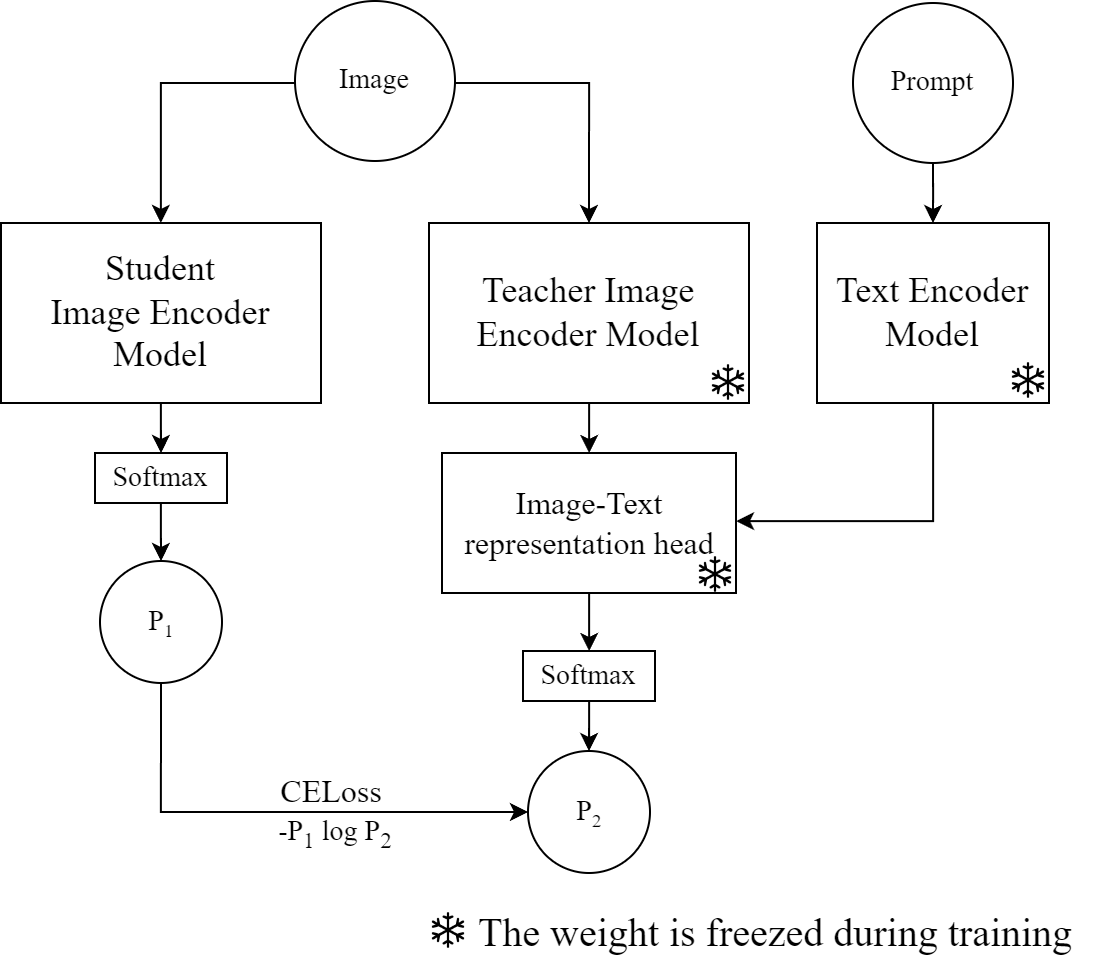
\includegraphics[width=0.75\textwidth]{Images/OverviewMethod.png}
    \end{center}
    \small
\end{figure}

By merging the two paradigms, we proposed a new approach to train an image classification model by distilling knowledge from a multimodal teacher as shown in Figure~\ref{fig:overall_method}.
Multimodal teacher models were constructed by leveraging a pre-trained language model and a pre-trained image encoder.
The output of both encoders was combined using cross-attention and a linear classification layer, called ``image-text representation head".
The detail of the image-text representation head is described in Figure~\ref{fig:cross_attention}.
In this work, the encoded text was used as a query to extract the relevant information from the image encoding.
The student model, which had the same architecture as the teacher image encoder model, was trained using teacher output as a target.
Thus, the student learned with high-level semantic information.

The result showed that by combining textual information with images, our approach improved accuracy by 3\% in both ResNet \shortcite{he2016deep} and ViT \shortcite{dosovitskiy2021an} model compared to the baseline self-distillation method.
The ablation study showed that the student model achieved 3\% higher accuracy by providing detailed descriptions in the training process.
This suggested that by using the text encodings with cross-attention, the model extracted higher semantic information and more precise image representations from the images.
% By repeating our self-distillation method, the accuracy of the student model gradually increases over each repetition.
% Ablation Image-text retrieval

To summarize our contribution.
Firstly this paper investigated the effectiveness of combining text-image representation by using text as a query to emphasize image representation in the self-distillation method.
Secondly, this work proposed a method to efficiently combine textual information and images for the self-distillation method.
Lastly, this work also investigated the effect of prompts in our methods to create image descriptions for training.

% The experimental is designed to answer the question of whether the joining of textual information with image representations to create joined text image representation can enhance both the training efficiency and the accuracy of the image classification model. Furthermore, the study investigates the potential benefits of leveraging the CLIP model’s ability to understand and utilize multimodal information.

% To summarize our contribution, Firstly this work propose a way to efficiently train text image representation header for self-distillation using teacher-student method. Secondly, this paper investigate the effectiveness of using text-image representation in a student-teacher framework. Lastly, this paper also investigate the effect of prompt using image captioning model as a image description text.

% Semi-supervised learning in image classification is a powerful approach that combines the advantages of both supervised and unsupervised learning. In recent studies focusing on semi-supervised learning for image classification, a popular strategy involves employing a teacher-student framework to generate pseudo-labels for training the student model. Notable examples of such frameworks include the $\Pi$-Model, Temporal Ensemble \shortcite{laine2016temporal}, Mean Teacher \shortcite{tarvainen2017mean} and EMAN Teacher \shortcite{cai2021exponential}. To improve the accuracy of the pseudo-labels, consistency regularization techniques have been widely adopted. These techniques, including mixup \shortcite{zhang2017mixup}, MixMatch \shortcite{berthelot2019mixmatch}, RandAugment \shortcite{cubuk2020randaugment}, FixMatch \shortcite{sohn2020fixmatch}, Interpolation Consistency Training \shortcite{verma2022interpolation} have been used by adding noise to image and image augmentation. Subsequently, two distinct views of the augmented images are fed into the teacher-student models, which are then trained to generate consistent outputs.v 

%However, the current self-distillation methods do not utilize textual information to create soft-label for a student model. With the textual information which is concise and informative, CLIP model \shortcite{radford2021learning} and Align \shortcite{jia2021scaling} has showed competitive performance compare to fully supervised image classification with zero-shot classification by utilize textual information using contrastive vision language pre-training method.

% The student-teacher framework for image classification using semi-supervised learning has attracted lot of interests, such as, EMA-teacher \shortcite{cai21eman}, EMAN \shortcite{cai21eman} and FixMatch \shortcite{DBLP:journals/corr/abs-2001-07685}. In such student-teacher framework, the teacher is first trained with the available labeled dataset as well as its augmented version.   Then through the teacher, pseudo-labeled datasets are generated for the students to learn.  

% This paper propose method to distill knowledge from both language encoder and vision encoder model from CLIP to create a classification model, which is need only image modal to do classification with specific number of classes. By distill knowledge from CLIP model, the student model will learn the knowledge which are summarized from CLIP model. This paper experiment with zero-shot learning and few-shot learning compare to CLIP model. This paper also compare the accuracy of student model and pretrained ViT \shortcite{dosovitskiy2021image} model in few-shot learning task.

% Knowledge distillation in image classification task have been investigated and showed performance increasing by using a student model with the same parameters size as a teacher model and difference parameters initialization, which is called self-distillation\shortcite{furlanello2018born, zhang2019your, xie2020self}. DINO \shortcite{caron2021emerging} also showed the performance increasing with both ResNet \shortcite{he2016deep} and Vision Transformers (ViT) \shortcite{dosovitskiy2021an} by using self-distillation without any label. \shortciteA{allen-zhu2023towards} has explained self-distillation that by training using self-distillation method, the student model is forced to learn all the features which the teacher model extracted from the datasets as a soft label target.